\documentclass{scrartcl} % scrartcl of scrreprt
% Include all project wide packages here.
\usepackage{fullpage}
\usepackage{polyglossia}
\setmainlanguage{dutch}
\usepackage{csquotes}
\usepackage{graphicx}
\usepackage{epstopdf}
\usepackage{pdfpages}
\usepackage{caption}
\usepackage[list=true]{subcaption}
\usepackage{float}
%\usepackage{mathtools}
\usepackage{standalone}
\usepackage{import}
\usepackage{tocloft}
\usepackage{wrapfig}
\usepackage{authblk}
\usepackage{array}
\usepackage{booktabs}
\usepackage[toc,page,title,titletoc]{appendix}
\usepackage{xunicode}
\usepackage{amsmath}
\usepackage{fontspec}
\usepackage{unicode-math}
\usepackage[
    backend=bibtexu,
	texencoding=utf8,
bibencoding=utf8,
    style=ieee,
    sortlocale=nl_NL,
    language=auto
]{biblatex}
\usepackage{listings}
\newcommand{\includecode}[3][c]{\lstinputlisting[caption=#2, escapechar=, style=#1]{#3}}
\newcommand{\superscript}[1]{\ensuremath{^{\textrm{#1}}}}
\newcommand{\subscript}[1]{\ensuremath{_{\textrm{#1}}}}


\newcommand{\chapternumber}{\thechapter}
\renewcommand{\appendixname}{Bijlage}
\renewcommand{\appendixtocname}{Bijlagen}
\renewcommand{\appendixpagename}{Bijlagen}

\usepackage[hidelinks]{hyperref} %<--------ALTIJD ALS LAATSTE

\renewcommand{\familydefault}{\sfdefault}

\setmainfont[Ligatures=TeX]{Myriad Pro}
\setmathfont{Asana Math}
\setmonofont{Lucida Console}

\usepackage{titlesec, blindtext, color}
\definecolor{gray75}{gray}{0.75}
\newcommand{\hsp}{\hspace{20pt}}
\titleformat{\chapter}[hang]{\Huge\bfseries}{\chapternumber\hsp\textcolor{gray75}{|}\hsp}{0pt}{\Huge\bfseries}
\renewcommand{\familydefault}{\sfdefault}
\renewcommand{\arraystretch}{1.2}
\setlength\parindent{0pt}

%For code listings
\definecolor{black}{rgb}{0,0,0}
\definecolor{browntags}{rgb}{0.65,0.1,0.1}
\definecolor{bluestrings}{rgb}{0,0,1}
\definecolor{graycomments}{rgb}{0.4,0.4,0.4}
\definecolor{redkeywords}{rgb}{1,0,0}
\definecolor{bluekeywords}{rgb}{0.13,0.13,0.8}
\definecolor{greencomments}{rgb}{0,0.5,0}
\definecolor{redstrings}{rgb}{0.9,0,0}
\definecolor{purpleidentifiers}{rgb}{0.01,0,0.01}


\lstdefinestyle{csharp}{
language=[Sharp]C,
showspaces=false,
showtabs=false,
breaklines=true,
showstringspaces=false,
breakatwhitespace=true,
escapeinside={(*@}{@*)},
columns=fullflexible,
commentstyle=\color{greencomments},
keywordstyle=\color{bluekeywords}\bfseries,
stringstyle=\color{redstrings},
identifierstyle=\color{purpleidentifiers},
basicstyle=\ttfamily\small}

\lstdefinestyle{c}{
language=C,
showspaces=false,
showtabs=false,
breaklines=true,
showstringspaces=false,
breakatwhitespace=true,
escapeinside={(*@}{@*)},
columns=fullflexible,
commentstyle=\color{greencomments},
keywordstyle=\color{bluekeywords}\bfseries,
stringstyle=\color{bluestrings},
identifierstyle=\color{purpleidentifiers}
}

\lstdefinestyle{vhdl}{
language=VHDL,
showspaces=false,
showtabs=false,
breaklines=true,
showstringspaces=false,
breakatwhitespace=true,
escapeinside={(*@}{@*)},
columns=fullflexible,
commentstyle=\color{greencomments},
keywordstyle=\color{bluekeywords}\bfseries,
stringstyle=\color{redstrings},
identifierstyle=\color{purpleidentifiers}
}

\lstdefinestyle{xaml}{
language=XML,
showspaces=false,
showtabs=false,
breaklines=true,
showstringspaces=false,
breakatwhitespace=true,
escapeinside={(*@}{@*)},
columns=fullflexible,
commentstyle=\color{greencomments},
keywordstyle=\color{redkeywords},
stringstyle=\color{bluestrings},
tagstyle=\color{browntags},
morestring=[b]",
  morecomment=[s]{<?}{?>},
  morekeywords={xmlns,version,typex:AsyncRecords,x:Arguments,x:Boolean,x:Byte,x:Char,x:Class,x:ClassAttributes,x:ClassModifier,x:Code,x:ConnectionId,x:Decimal,x:Double,x:FactoryMethod,x:FieldModifier,x:Int16,x:Int32,x:Int64,x:Key,x:Members,x:Name,x:Object,x:Property,x:Shared,x:Single,x:String,x:Subclass,x:SynchronousMode,x:TimeSpan,x:TypeArguments,x:Uid,x:Uri,x:XData,Grid.Column,Grid.ColumnSpan,Click,ClipToBounds,Content,DropDownOpened,FontSize,Foreground,Header,Height,HorizontalAlignment,HorizontalContentAlignment,IsCancel,IsDefault,IsEnabled,IsSelected,Margin,MinHeight,MinWidth,Padding,SnapsToDevicePixels,Target,TextWrapping,Title,VerticalAlignment,VerticalContentAlignment,Width,WindowStartupLocation,Binding,Mode,OneWay,xmlns:x}
}

%defaults
\lstset{
basicstyle=\ttfamily\small,
extendedchars=false,
numbers=left,
numberstyle=\ttfamily\tiny,
stepnumber=1,
tabsize=4,
numbersep=5pt
}
\addbibresource{../../library/bibliography.bib}

\author{Xenia Wesdijk \and Robin Hes}
\title{EPO3: Eindrapport - SPI}

\begin{document}
\chapter{SPI}
\label{ch:spi}

%specificaties
\section{Specificaties}
Voor de communicatie tussen de arduino en onze GPU is een protocol nodig. Er is gekozen deze communicatie met SPI af te handelen. Een simpele specificatie voldoet, aangezien er alleen data ontvangen hoeft te worden en er maar één SPI-slave in het systeem aanwezig is. In figuur~\ref{fig:spi-schema} is te zien welke in- en uitgangen de SPI-module dient te hebben.

\begin{figure}[H]
	\centering
	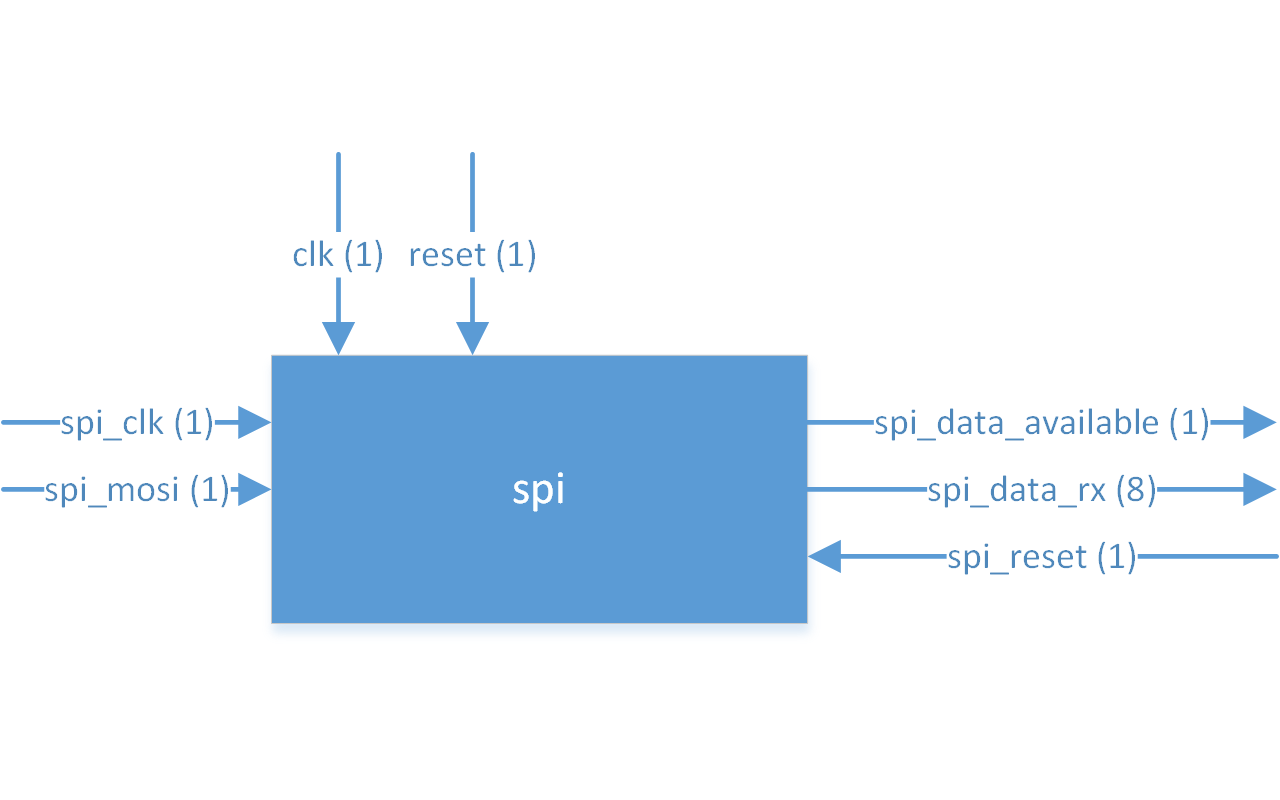
\includegraphics[width=\textwidth]{resource/spi.png}
	\caption{Een blokschema van de SPI-module, met de namen van de gebruikte in- en uitgangen en tussen haakjes het aantal bits}
	\label{fig:spi-schema}
\end{figure}

Naast het algemene kloksignaal heeft de SPI zijn eigen kloksignaal (SCLK). Op iedere rijzende klokfland van dit signaal moet het bit dat op de MOSI ingang staat gelezen worden. Nadat er acht opeenvolgende bits gelezen zijn (en byte), moet het signaal spi\_data\_ready omhoog, waarbij tegelijker tijd de acht gelezen bits als een byte op de spi\_data\_rx komen te staan.

%Ontwerp & implementatie
\section{Ontwerp en implementatie}
De SPI-module is vrij simpel en bestaat eigenlijk alleen uit een stuk logica wat de inkomende bits synchroniseert met het systeemwijde kloksignaal, en een shift-register om waarin uit de acht ontvangen bits een byte gevormd wordt. Helaas zijn we er in de praktijk niet in geslaagd een SPI-module te maken die helemaal stabiel was. De reden is onbekend, maar de module gaat relatief vaak out-of-sync tijdens het ontvangen van een byte, waardoor de module 'denkt' dat hij al een gehele byte ontvangen heeft, waar dat in werkelijkheid slechts zeven bits zijn. Om dit probleem te verzachten zit er een extra reset in de module, alsmede een timer die de module reset, wanneer hij dreigt vast te lopen.

%VHDL simulatie
\section{VHDL simulatie}
Allereerst is er een simulatie gemaakt met behulp van ModelSim. In de testbench die geschreven is voor de SPI module wordt één byte ontvangen. Zoals te zien in figuur~\ref{fig:spi-modelsim}, wordt het laatst via MOSI ontvangen bit inderdaad toegevoegd aan het signaal spi\_data\_rx. Wanneer op deze manier 8-bits ontvangen zijn gaat het signaal spi\_data\_available op hoog, om aan te geven dat er gelezen kan worden.

\begin{figure}[H]
	\centering
	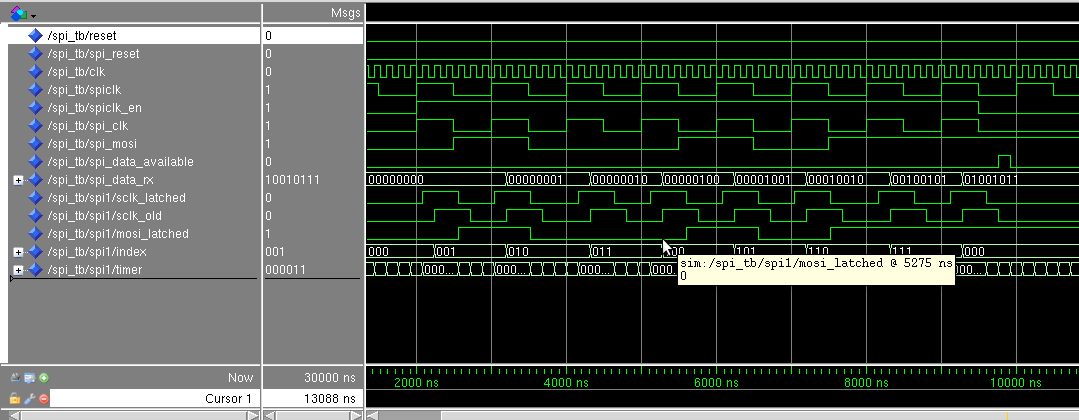
\includegraphics[width=\textwidth]{resource/waveSPI2.png}
	\caption{Een fragment van de wave van de SPI module}
	\label{fig:spi-modelsim}
\end{figure}

%Synthese
\section{Synthese en lay-out}
\label{sec:spi-synth} 
Na uitvoering van de synthese op de SPI module blijkt dat de SPI een redelijk compacte module is. Door bij de synthese gebruik te maken van compile\_ultra verkregen we een totaal celloppervlak van 695 transistoren. Na met row placer handmatig de cellen te hebben geplaatst, hierbij is de optie "vary distance'' uitgeschakeld, leverde de lay-out met trout een totaal van 2630 transistoren op. Van deze transistoren worden er een aantal van 1385 transistoren daadwerkelijk gebruikt. Dit levert een efficiëntie op van 52.66\%.

%Switchlevel test
\section{Switch-level simulatie}
De switch-level simulatie vergelijkt de simulatie op het transistor niveau met de simulatie op VHDL niveau. De resultaten van de gesynthetiseerde schakeling, die gesimuleerd is met SLS, wordt vergeleken met de resultaten van de gesimuleerde testbench in ModelSim. Het verkregen switch-level resultaat, zie figuur \ref{fig:spi-sls}, komt overeen met het al eerder verkregen ModelSim resultaat. Ook is er nog gebruik gemaakt van de optie compare. Deze leverde het verwachte resultaat. Hieruit kunnen we concluderen dat de synthese van de SPI module goed is verlopen. 

\begin{figure}[H]
	\centering
	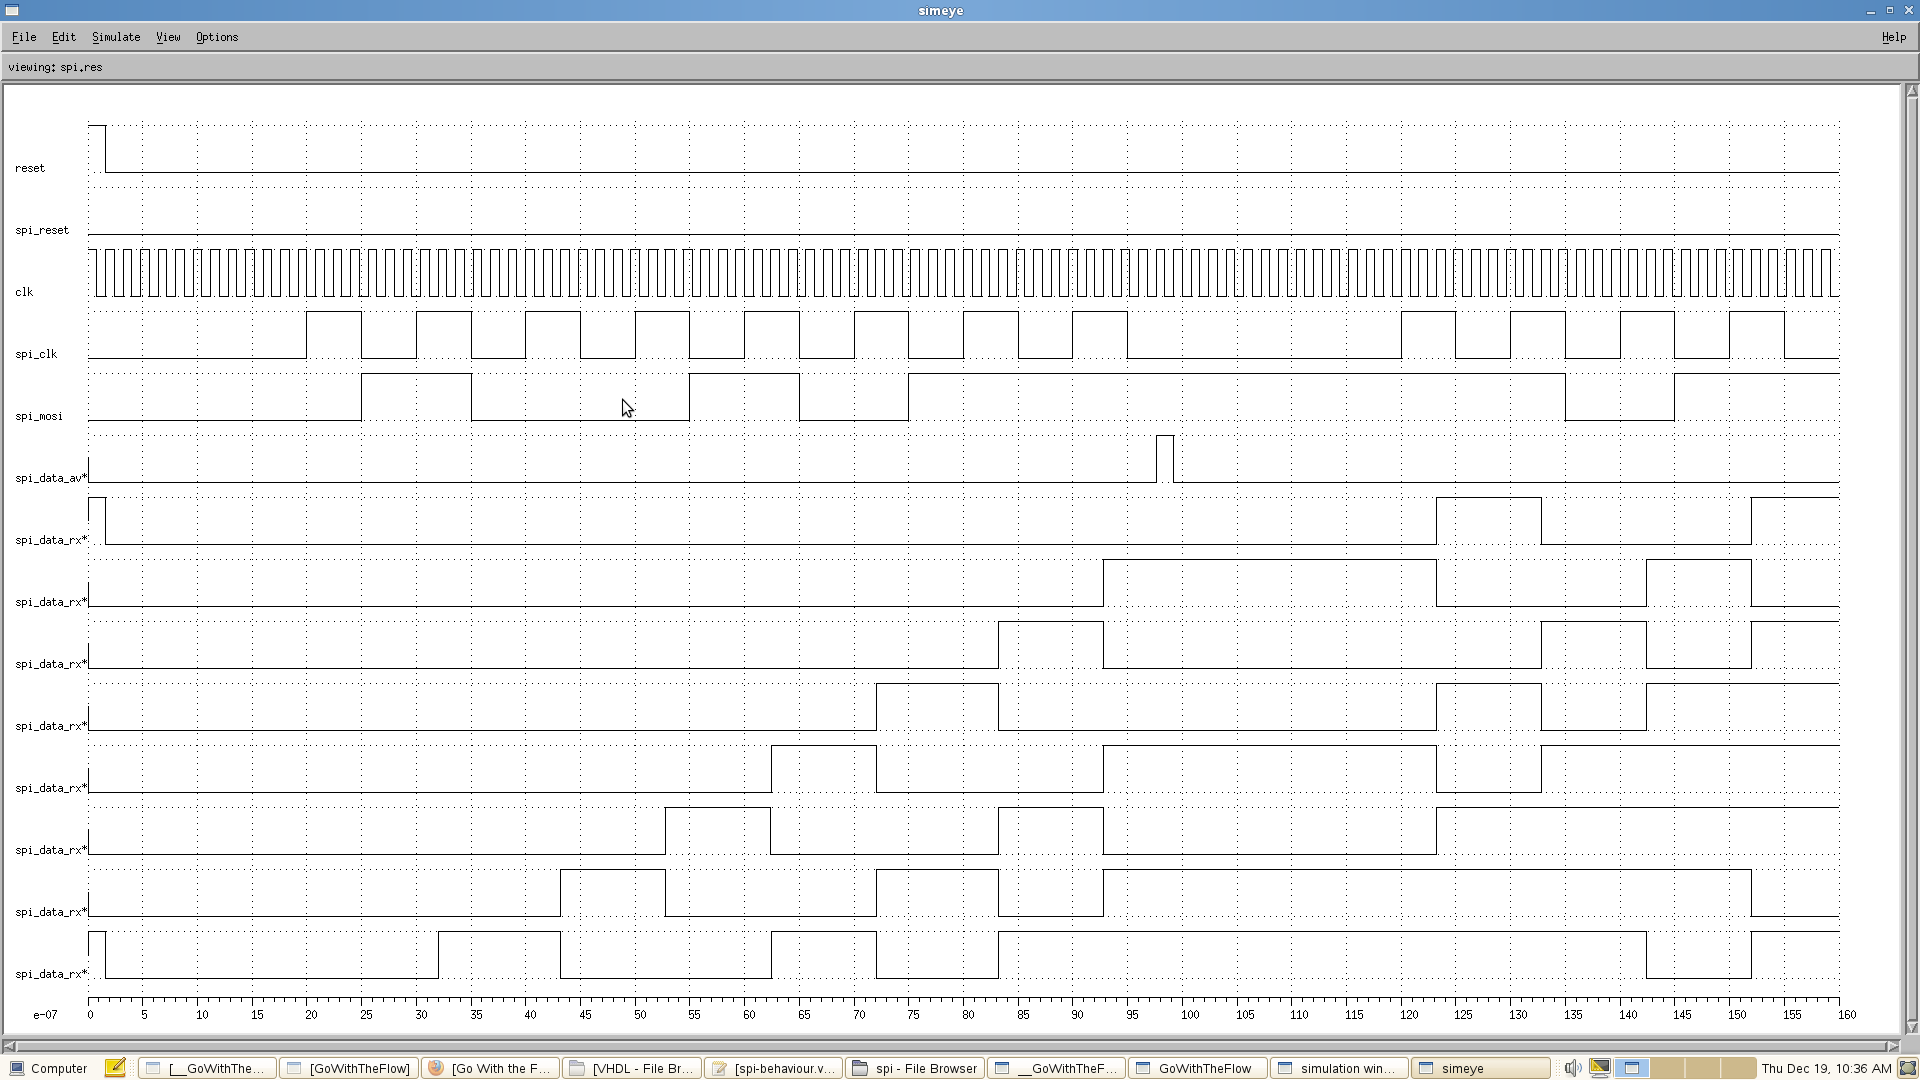
\includegraphics[width=\textwidth]{resource/switchlevelSPI.png}
	\caption{Het switch-level resultaat van de SPI module}
	\label{fig:spi-sls}
\end{figure}

%Conclusie AF
\section{Conclusie}
Alle gemaakte simulaties van de SPI module leverde uiteindelijk het gewenste resultaat op.
Naar aanleiding hiervan kan dan dus de conclusie worden getrokken dan de SoG-implementatie van de module goed is en een werkend resultaat op zou moeten leveren.

De VHDL beschrijving en testbench staan in Bijlagen \ref{appsec:spi.vhd}, \ref{appsec:spi-behaviour.vhd}, \ref{appsec:spi-tb.vhd} en \ref{appsec:spi-tb-behaviour.vhd}.

\end{document}
